\documentclass[a4paper,12pt,oneside,openany,table,xcdraw]{article}

\usepackage{setspace}
\usepackage{multirow}
\usepackage{hyperref}
\usepackage{caption}
\usepackage{indentfirst}
\usepackage{tikz} %% fasores
\usetikzlibrary{arrows,arrows.meta,quotes,angles}
\usepackage{siunitx}

\usepackage[brazilian]{babel}
\usepackage[utf8x]{inputenc}
\usepackage{amsmath, graphicx, subfig, enumerate}
\usepackage{float, verbatim}
\usepackage[colorinlistoftodos]{todonotes}
\usepackage{makeidx}
\usepackage{geometry}

\graphicspath{{img/}}
\geometry{a4paper, hmargin={3cm, 3cm}, vmargin={3cm, 2cm} }
\setlength{\parindent}{1.0cm}
\captionsetup{font=small}

\begin{document}
\newcommand{\thedepartment}{Faculdade de Engenharia Elétrica}
\newcommand{\thecourse}{FEELT}
\newcommand{\thetitle}{VERIFICAÇÃO DA SEQUÊNCIA DE FASES DAS TENSÕES}
\newcommand{\thetype}{Relatório da Disciplina de Experimental de Circuitos Elétricos II}
\newcommand{\theproftitle}{Bacharel em Engenharia Elétrica}
\newcommand{\thestudent}{Lesly Viviane Montúfar Berrios\\
\centering11811ETE001}
\newcommand{\theadvisor}{Prof. Wellington Maycon Santos Bernardes}
\newcommand{\thecity}{Uberlândia}

\thispagestyle{empty}\newcommand*{\themonth}{\ifthenelse{\the\month < 2}{Janeiro }
                  {\ifthenelse{\the\month < 3}{Fevereiro }
                  {\ifthenelse{\the\month < 4}{Março }
                  {\ifthenelse{\the\month < 5}{Abril }
                  {\ifthenelse{\the\month < 6}{Maio }
                  {\ifthenelse{\the\month < 7}{Junho }
                  {\ifthenelse{\the\month < 8}{Julho }
                  {\ifthenelse{\the\month < 9}{Agosto }
                  {\ifthenelse{\the\month < 10}{Setembro }
                  {\ifthenelse{\the\month < 11}{Outubro }
                  {\ifthenelse{\the\month < 12}{Novembro }{Dezembro }}}}}}}}}}}}
                  
\begin{titlepage}
\begin{center}

	\vspace{-0.5cm}

  \begin{figure}[hbt!]
		\begin{center}
		   
\includegraphics[width=2.8cm]{ufu-logo.png}
		\end{center}
	\end{figure}
 	%\vspace{-4cm}

%\begin{doublespacing}

  \Large{\textbf{Universidade Federal de Uberlândia}}\\
  \large{\thedepartment}\\
  \large{\thecourse}\\


\vspace{5.8cm}
  \par
  \large\textbf{\thetitle}
\vspace{5.8cm} 

%\end{doublespacing}
  \par
  \thetype\\
  por\\
  %\hspace{2cm}\large{}\\

\vspace{0.8cm}
\par
  \normalsize{\thestudent}\\ [2cm]
  \theadvisor

\par\vfill
  \thecity, \themonth / \the\year

\end{center}

\end{titlepage}

%% Comeca o documento !

\onehalfspacing
\tableofcontents % sumário
\newpage

\section{Objetivos} % 2,5%
Pretende-se verificar experimentalmente conceitos teóricos de como encontrar a correta sequência de
fase diante da ausência de um sequencímetro (método do voltímetro).

\section{Introdução teórica} % 5%

O sequencímetro é um instrumento de medida elétrica analógica ou digital que tem por  finalidade a verificação da sequência de fases de um motor trifásico (circuito alimentado por corrente alternada), ou seja, indica a fase aberta e o sentido de rotação do motor. Na Figura \ref{intro:fig1}, é observado um fasímetro, que possui a mesma função, havendo poucas diferenças, entre elas, estão a tensão de entrada e a faixa de frequência. Sobre seu funcionamento diz-se que, a partir do momento em que o sequencímetro detecta a passagem por zero (pulso positivo de curta duração) de cada fase é aplicado em um circuito sequencial feito com flip-flop e indica a sequência da rede \cite{UNIR}.

Na ausência desse tipo de equipamento, circuitos desequilibrados podem ser utilizados para a verificação de sequência de fases em certo sistema elétrico. Basendo-se na queda de tensão em cada fase, é possível provar matematicamente qual é a sequência de fases utilizada, por meio da análise do circuito, sendo os resultados teóricos dispostos na Sessão \ref{dados}.

\vspace{0.5cm}
\begin{figure}[H]
\centering
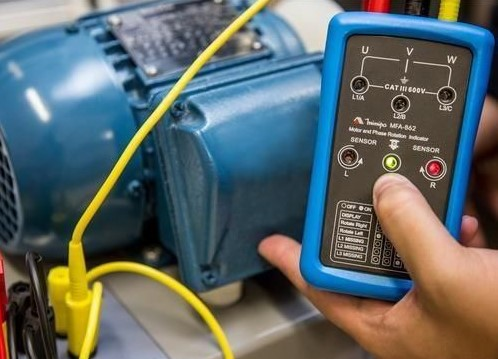
\includegraphics[width=12.5cm]{fasimetro}
\caption{Fasímetro com indicador led 690 volts - MFA-862 \cite{fig1}.}
\label{intro:fig1}
\end{figure}
\vspace{0.3cm}


\section{Preparação}
\subsection{Materiais e ferramentas} % 2,5%
\begin{enumerate}[1 -]
\item \emph{\textbf{Fonte:}}
Alimentará todo o circuito. Possui frequência de $60\ Hz$.

\item \emph{\textbf{Regulador de tensão (Varivolt):}}
Também chamado de autotransformador, permitirá obter o valor desejado de corrente a partir da regulagem correta da tensão fornecida pela fonte.

\item \emph{\textbf{Conectores:}}
Para as conexões no circuito foi utilizado majoritariamente cabos banana-banana.

\item \emph{\textbf{Medidor eletrônico KRON Mult K:}}
Possibilita encontrar a medição da potência real (P) - vatímetro, reativa (Q) e aparente (S) do circuito. Ele também possui função de cofasímetro, instrumento elétrico que mede o fator de potência (fp, $cos\theta$) ou o ângulo da impedância $\theta$ do circuito, para um circuito com a impedância $Z = Z\angle \theta$.

\item \emph{\textbf{Resistor de $50\Omega$:}}
Carga resistiva para compor a carga do circuito trifásico.

\item \emph{\textbf{Capacitor de $45,9\mu F$:}}
Sendo sua resistência quase nula, portanto desprezível nessa aplicação (Esquenta pouco, logo dissipa menos energia).
\end{enumerate}

\vspace{0.2cm}
\subsection{Montagem} % 2,5%

\subsubsection{Verificação da sequência de fases}
A montagem para o método do voltímetro pode ser realizado por meio de voltímetros analógicos, como mostra a Figura \ref{m1:analogico}, ou mediante equipamento digital, como na Figura \ref{m1:esquema}. Para este experimento utilizou o medidor digital \emph{Kron}, com configuração TL=0000 (Trifásico Equilibrado ou Desequilibrado Estrela - 3F + N - 3 elementos 4 fios). 
Assim, no caso de equipamento digital, aplica-se uma tensão linha $V_L=100V$ com o auxílio do \emph{Varivolt}, em frequência de 60Hz, e parâmetros de carga: $R=50\Omega$ e $C=45,9 \mu F$. Ademais, como procedimento de segurança, é verificado sempre se existe algum curto-circuito em alguma das fases em baixa tensão.

\vspace{0.2cm}
\begin{figure}[H]
\centering
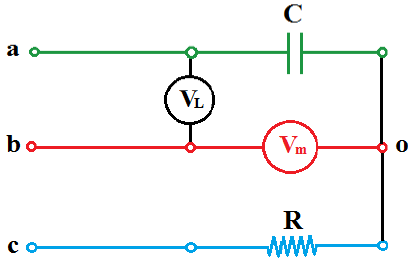
\includegraphics[width=11.5cm]{m-analog}
\caption{Método do voltímetro, utilizando-se voltímetros analógicos.}
\label{m1:analogico}
\end{figure}

\vspace{2cm}
\begin{figure}[H]
\centering
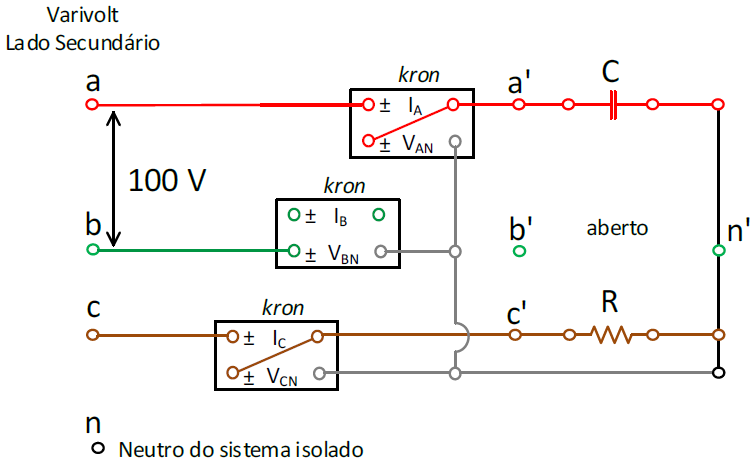
\includegraphics[width=13cm]{m1-circuito}
\caption{Método do voltímetro, utilizando-se equipamento digital.}
\label{m1:esquema}
\end{figure}

\newpage
\subsubsection{Verificação da sequência de fases - Fase A aberta}
A primeira montagem com a fase A aberta resulta na montagem da Figura \ref{m2:esquema}.
\vspace{0.3cm}
\begin{figure}[H]
\centering
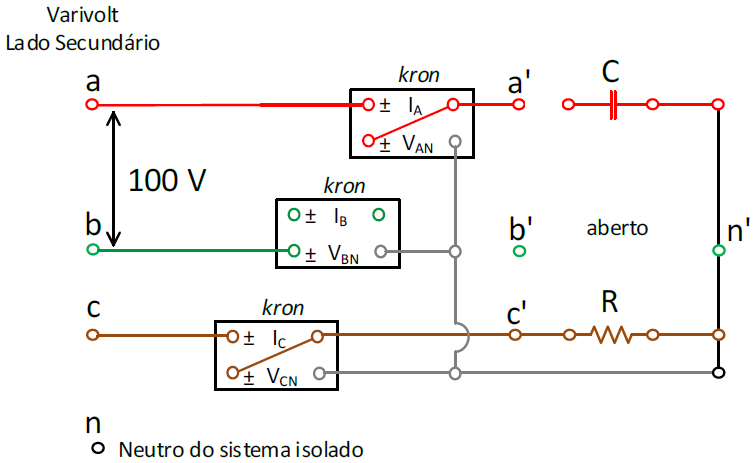
\includegraphics[width=13cm]{m2-circuito}
\caption{Montagem 1 com fase A aberta.}
\label{m2:esquema}
\end{figure}
\vspace{0.1cm}

\subsubsection{Verificação da sequência de fases - Fase C aberta}
A primeira montagem com a fase C aberta resulta na montagem da Figura \ref{m3:esquema}.
\vspace{0.3cm}
\begin{figure}[H]
\centering
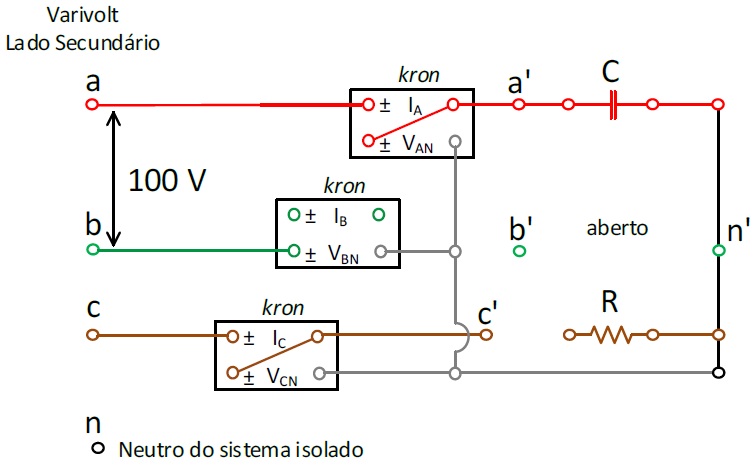
\includegraphics[width=13cm]{m3-circuito}
\caption{Montagem 1 com fase C aberta.}
\label{m3:esquema}
\end{figure}
\vspace{0.1cm}

\newpage
\section{Dados Experimentais} \label{dados}
Embora, esta sessão seja reservada para os dados obtidos experimentalmente, também são comptemplados, nas tabelas que seguem, os resultados teóricos.

\subsubsection{Verificação da sequência de fases}
Da análise teórica do circuito, determina-se ainda os fasores teóricos $I_{ac}$ e $I_{bn'}$, para assim compará-lo com o dado experimental, conforme a Tabela \ref{m1:dados}. Ademais, a partir dos fasores determinados da teoria, desenha-se os fasores de tensão e corrente para cada caso, como na Figura \ref{m1:fasores}. Vale lembrar que os fasores estão escalados de diferentes fatores para melhor visualização.
\vspace{-0.4cm}

\begin{equation*}
\begin{array}{l}
Z_{A} =j\ \dfrac{1}{2\pi \cdot 60\cdot 45,9\mu } =-j\ 57,79\ [ \si{\Omega}]\\
\\
Z_{C} =50\ [ \si{\Omega}]\\
\\
57,74\angle 0\mathrm{^{\circ }} -( 50-j\ 57,79) \ I_{A} =54,74\angle 120\mathrm{^{\circ }}\\
\\
I_{A} =\dfrac{57,74\angle 0\mathrm{^{\circ }} -57,74\angle 120\mathrm{^{\circ }}}{50-j\ 57,79} =1,309\angle 19,13\mathrm{^{\circ }}\\
\\
V_{n'} =57,74\angle 0\mathrm{^{\circ }} +j\ 57,79\cdot I_{A} =78,68\angle 65,24\mathrm{^{\circ }}\\
V_{b'n'} =V_{b'} -V_{n'} =54,74\angle -120\mathrm{^{\circ }} -78,68\angle 65,24\mathrm{^{\circ }} =136,3\angle -117\mathrm{^{\circ }}
\end{array}
\end{equation*}

\vspace{0.4cm}
O cálculo é análogo para a fase CBA, assim tem-se:
\vspace{-0.4cm}

\begin{equation*}
\centering
\begin{aligned}
\mathrm{\begin{bmatrix}
I_{ac}\\
V_{bn'}
\end{bmatrix}} =\mathrm{\begin{bmatrix}
1,309\angle 19,13\mathrm{^{\circ }}\\
136,3\angle -117,0\mathrm{^{\circ }}
\end{bmatrix}} & \text{  para ABC e} & \mathrm{\begin{bmatrix}
I_{ac}\\
V_{bn'}
\end{bmatrix}} =\mathrm{\begin{bmatrix}
1,309\angle 79,13\mathrm{^{\circ }}\\
37,82\angle 109,0\mathrm{^{\circ }}
\end{bmatrix}} & \text{  para CBA.}
\end{aligned}
\end{equation*}

\vspace{0.4cm}
\begin{table}[H]
\centering \small \def\arraystretch{1.32}
\caption{Verificação da sequência de fases}
\label{m1:dados}
\begin{tabular}{c|c|c|c|c|}
\cline{2-5}
\multicolumn{1}{l|}{} & \multicolumn{2}{c|}{Sequência abc} & \multicolumn{2}{c|}{Sequência cba} \\ \cline{2-5} 
 & $I_{ac}$ (A) & $V_{bn'}$ (V) & $I_{ac}$ (A) & $V_{bn'}$ (V) \\ \hline
\multicolumn{1}{|c|}{Teórico} & 1,309 & 136,3 & 1,309 & 37,82 \\ \hline
\multicolumn{1}{|c|}{Medido} & 1,297 & 139,7 & 1,277 & 39,10 \\ \hline
\multicolumn{1}{|c|}{Erro(\%)} & -0,917 & 2,494 & -2,445 & 3,384 \\ \hline
\end{tabular}
\end{table}
\vspace{0.3cm}

\begin{figure}[H]
\centering
    \begin{tikzpicture}[ > = angle 90, phasor/.style = {very thick,-{Triangle[fill=white]}}, angles/.style = {draw, <->, angle eccentricity=1, right, angle radius=7mm}]

    % coordinates
    \draw[->] (-2,0) -- (4,0) coordinate (x) node[below left] {$Re$};
    \draw[->] (0,-3.2) -- (0,2.5) node[below left] (y) {$Im$};

    % phasors
    \draw[phasor, red] (0,0) -- (19.13:1.297/1.8) coordinate (ia)  node[right] {$I_{ac}$};
    \draw[phasor, blue] (0,0) -- (-117:139.7/40) coordinate (va)  node[right] {$V_{bn'}$};

    \end{tikzpicture}\hfill
     \begin{tikzpicture}[ > = angle 90, phasor/.style = {very thick,-{Triangle[fill=white]}}, angles/.style = {draw, <->, angle eccentricity=1, right, angle radius=7mm}]
    
    % coordinates
    \draw[->] (-0.5,0) -- (4,0) coordinate (x) node[below left] {$Re$};
    \draw[->] (0,-3.2) -- (0,2.5) node[below left] (y) {$Im$};

     % phasors
    \draw[phasor, red] (0,0) -- (79.13:1.277/1.8) coordinate (ia)  node[right] {$I_{ac}$};
    \draw[phasor, blue] (0,0) -- (109:39.10/40) coordinate (va)  node[right] {$V_{bn'}$};

    \end{tikzpicture}
\caption{Diagrama fasorial para a montagem 1 em fase ABC e CBA respectivamente.}
\label{m1:fasores}
\end{figure}
\vspace{1cm}

\subsubsection{Verificação da sequência de fases - Fase A aberta}
Para o caso da fase A aberta, tem-se os dados experimentais da Tabela \ref{m2:dados}. Ainda da análise teórica determina-se $I_{ac}$ e $V_{bn'}$, para assim poder desenhar os fasores dessas grandezas, que encontram dispostos na Figura \ref{m2:fasores}. 
\vspace{-0.2cm}

\begin{equation*}
\begin{aligned}[c]
\mathrm{\begin{bmatrix}
I_{ac}\\
V_{bn'}
\end{bmatrix}} =\mathrm{\begin{bmatrix}
0\\
100\angle -90\mathrm{^{\circ }}
\end{bmatrix}} & \text{ \ para ABC e} & \mathrm{\begin{bmatrix}
I_{ac}\\
V_{bn'}
\end{bmatrix}} =\mathrm{\begin{bmatrix}
0\\
100\angle 90\mathrm{^{\circ }}
\end{bmatrix}} & \text{ \ para CBA.}
\end{aligned}
\end{equation*}

\vspace{0.6cm}
\begin{table}[H]
\centering \small \def\arraystretch{1.32}
\caption{Verificação da sequência de fases - fase A aberta}
\label{m2:dados}
\begin{tabular}{c|c|c|c|c|}
\cline{2-5}
\multicolumn{1}{l|}{} & \multicolumn{2}{c|}{Sequência ABC} & \multicolumn{2}{c|}{Sequência CBA} \\ \cline{2-5} 
 & $I_{AC}$ (A) & $V_{BN'}$ (V) & $I_{AC}$ (A) & $V_{BN'}$ (V) \\ \hline
\multicolumn{1}{|c|}{Teórico} & 0 & 100,0 & 0 & 100,0 \\ \hline
\multicolumn{1}{|c|}{Medido} & 0 & 102,2 & 0 & 101,7 \\ \hline
\multicolumn{1}{|c|}{Erro(\%)} & 0 & 2,2 & 0 & 1,7 \\ \hline
\end{tabular}
\end{table}
\vspace{0.3cm}

\begin{figure}[H]
\centering
    \begin{tikzpicture}[ > = angle 90, phasor/.style = {very thick,-{Triangle[fill=white]}}, angles/.style = {draw, <->, angle eccentricity=1, right, angle radius=7mm}]

    % coordinates
    \draw[->] (-0.5,0) -- (4,0) coordinate (x) node[below left] {$Re$};
    \draw[->] (0,-3) -- (0,3) node[below left] (y) {$Im$};

    % phasors
    \fill[red] (0,0) circle (0.8mm) node[right] {$I_{ac}$};
    \draw[phasor, blue] (0,0) -- (-90:102.2/40) coordinate (va)  node[right] {$V_{bn'}$};

    \end{tikzpicture}\hfill
     \begin{tikzpicture}[ > = angle 90, phasor/.style = {very thick,-{Triangle[fill=white]}}, angles/.style = {draw, <->, angle eccentricity=1, right, angle radius=7mm}]
    
    % coordinates
    \draw[->] (-0.5,0) -- (4,0) coordinate (x) node[below left] {$Re$};
    \draw[->] (0,-3) -- (0,3) node[below left] (y) {$Im$};

     % phasors
    \fill[red] (0,0) circle (0.8mm) node[right] {$I_{ac}$};
    \draw[phasor, blue] (0,0) -- (90:101.7/40) coordinate (va)  node[right] {$V_{bn'}$};

    \end{tikzpicture}
\caption{Diagrama fasorial para a montagem 2 em fase ABC e CBA respectivamente.}
\label{m2:fasores}
\end{figure}
\vspace{1cm}

\subsubsection{Verificação da sequência de fases - Fase C aberta}
Já para o caso da fase C aberta, tem-se os dados experimentais da Tabela \ref{m3:dados}. Ainda da análise teórica determina-se $I_{ac}$ e $V_{bn'}$, para assim poder desenhar os fasores dessas grandezas, que encontram dispostos na Figura \ref{m3:fasores}. 
\vspace{-0.2cm}

\begin{equation*}
\begin{aligned}[c]
\mathrm{\begin{bmatrix}
I_{ac}\\
V_{bn'}
\end{bmatrix}} =\mathrm{\begin{bmatrix}
0\\
100\angle -150\mathrm{^{\circ }}
\end{bmatrix}} & \text{ \ para ABC e} & \mathrm{\begin{bmatrix}
I_{ac}\\
V_{bn'}
\end{bmatrix}} =\mathrm{\begin{bmatrix}
0\\
100\angle 150\mathrm{^{\circ }}
\end{bmatrix}} & \text{ \ para CBA.}
\end{aligned}
\end{equation*}

\vspace{1cm}
\begin{table}[H]
\centering \small \def\arraystretch{1.32}
\caption{Verificação da sequência de fases - fase C aberta}
\label{m3:dados}
\begin{tabular}{c|c|c|c|c|}
\cline{2-5}
\multicolumn{1}{l|}{} & \multicolumn{2}{c|}{Sequência ABC} & \multicolumn{2}{c|}{Sequência CBA} \\ \cline{2-5} 
 & $I_{ac}$ (A) & $V_{bn'}$ (V) & $I_{ac}$ (A) & $V_{bn'}$ (V) \\ \hline
\multicolumn{1}{|c|}{Teórico} & 0 & 100,0 & 0 & 100,0 \\ \hline
\multicolumn{1}{|c|}{Medido} & 0 & 100,4 & 0 & 101,0 \\ \hline
\multicolumn{1}{|c|}{Erro(\%)} & 0 & 0,4 & 0 & 1,0 \\ \hline
\end{tabular}
\end{table}

\begin{figure}[H]
\centering
    \begin{tikzpicture}[ > = angle 90, phasor/.style = {very thick,-{Triangle[fill=white]}}, angles/.style = {draw, <->, angle eccentricity=1, right, angle radius=7mm}]

    % coordinates
    \draw[->] (-2.5,0) -- (2,0) coordinate (x) node[below left] {$Re$};
    \draw[->] (0,-2) -- (0,3) node[below left] (y) {$Im$};

    % phasors
    \fill[red] (0,0) circle (0.8mm) node[right] {$I_{ac}$};
    \draw[phasor, blue] (0,0) -- (-150:100.4/40) coordinate (va)  node[right] {$V_{bn'}$};

    \end{tikzpicture}\hfill
     \begin{tikzpicture}[ > = angle 90, phasor/.style = {very thick,-{Triangle[fill=white]}}, angles/.style = {draw, <->, angle eccentricity=1, right, angle radius=7mm}]
    
    % coordinates
    \draw[->] (-2.5,0) -- (2,0) coordinate (x) node[below left] {$Re$};
    \draw[->] (0,-2) -- (0,3) node[below left] (y) {$Im$};

     % phasors
    \fill[red] (0,0) circle (0.8mm) node[right] {$I_{ac}$};
    \draw[phasor, blue] (0,0) -- (150:101.0/40) coordinate (va)  node[right] {$V_{bn'}$};

    \end{tikzpicture}
\caption{Diagrama fasorial para a montagem 3 em fase ABC e CBA respectivamente.}
\label{m3:fasores}
\end{figure}
\vspace{0.2cm}


\section{Análise sobre segurança} % 2,5%
Os óculos de segurança são Equipamentos de Proteção Individual (EPIs) e são utilizados para a proteção da área ao redor dos olhos contra qualquer tipo de detrito estranho, que possa causar irritação ou ferimentos. Também protegem contra faíscas, respingos de produtos químicos, detritos, poeira, radiação e etc \cite{safe}.
É importante a utilização desse equipamento durante os experimentos a fim de evitar qualquer dano, além de preparar o profissional para o manejo correto e seguro de qualquer equipamento.
Além disso, foi de extrema importância a presença do professor ou técnico na verificação da montagem do circuito antes de energizá-lo. Assim, reduziu-se riscos de curtos-circuitos ou sobrecarga na rede.

\vspace{0.2cm}
\section{Reflexão} % (quando houver) (70%)
\subsubsection{E na ausência de um voltímetro?}
% - Na impossibilidade de ter voltímetros, amperímetros e sequencímetro, como você poderia encontrar a solução desse problema (abc ou cba)?
 Na ausência de voltímetros, amperímetros ou sequencímetro, pode-se utilizar equipamentos permitam de forma visual ou sensitiva identificar a fase com maior e maior tensão, para assim prosseguir com a análise realizada neste experimento. No caso de tensão na fase superior à tensão de linha aplicada a sequência de fases correspondente é ABC, enquanto que se for inferior, será sequência de fases CBA.
 Por exemplo, é possível verificar o mesmo efeito conectando-se lâmpadas aos terminais $V_{ab}$ e $V_{bn'}$ para assim constatar a ddp entre os terminais em que estão conectadas por meio da viasualização da intensidade do brilhar da lâmpada.
 
\subsubsection{Sobre a importância da sequência de fase em um circuito elétrico}
% - Aponte a importância de encontrar a correta sequência de fase em um circuito elétrico.
Saber a sequência de fase em um circuito desequilibrado é de grande importância. Para circuitos equilibrados, o efeito é mínimo, uma vez que os módulos das tensões e correntes de linha e de fase são idênticos, e há somente uma defasagem entre elas. No entanto, para cargas desequilibradas, que são mais comuns e trata-se de uma situação, é essencial conhecer a sequência de fases em que trabalha, seja para evitar danos em equipamentos conectados às fases ou determinar a direção de
rotação de uma motor de indução
conectado à fonte de tensão trifásica.

\vspace{1cm}
\section{Simulação computacional} % (10%);
Para a simulação foi utilizada uma fonte CBA, por isso pode haver alguma estranheza no circuito por parte do leitor. No entanto, a análise é a mesma.
\vspace{0.2cm}

\subsubsection{Verificação da sequência de fases}

\begin{figure}[H]
\centering
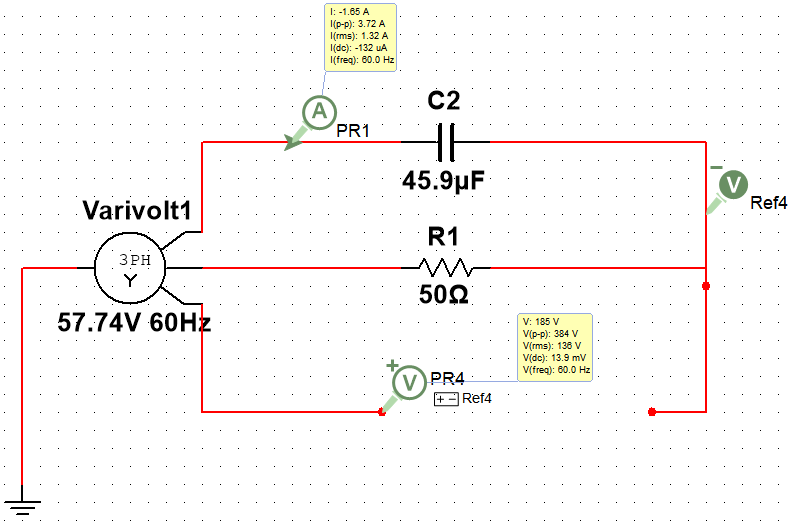
\includegraphics[width=13cm]{m1-sim-abc}
\caption{Método do voltímetro, utilizando-se equipamento digital.}
\label{m1:sim:abc}
\end{figure}

\vspace{0.2cm}
\begin{figure}[H]
\centering
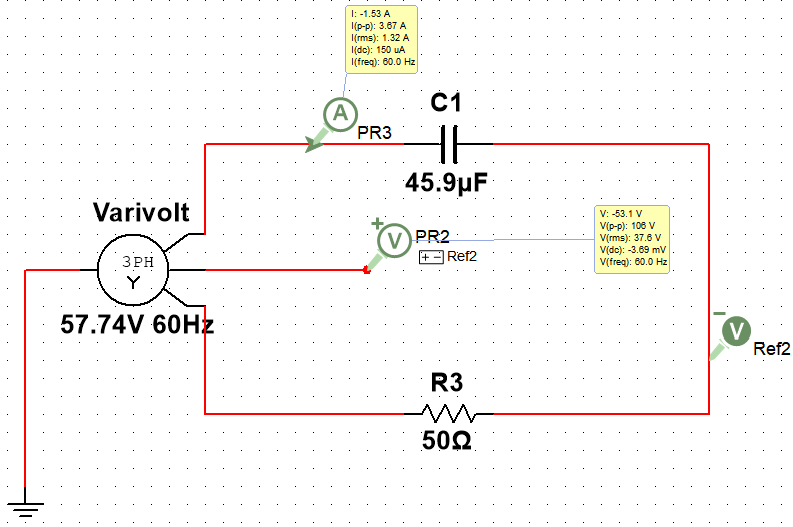
\includegraphics[width=13cm]{m1-sim-cba}
\caption{Simulação para determinação de sequência de fase CBA.}
\label{m1:sim:cba}
\end{figure}

\vspace{1cm}
\subsubsection{Verificação da sequência de fases - Fase A aberta}
\begin{figure}[H]
\centering
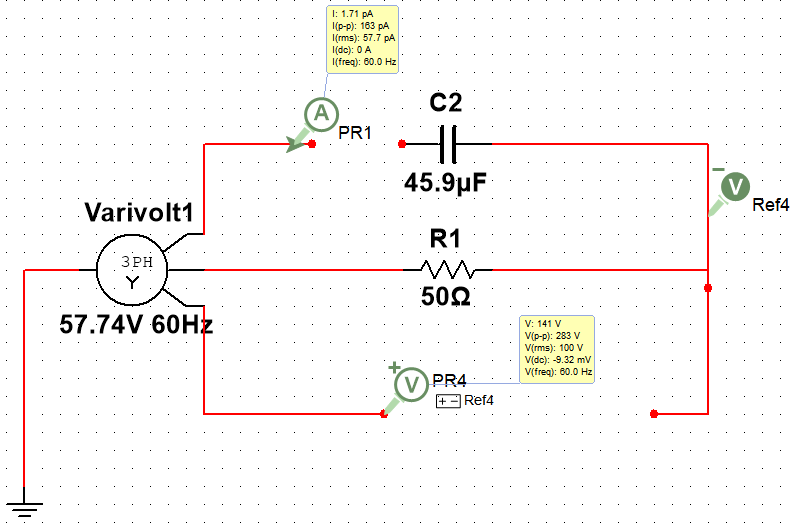
\includegraphics[width=13cm]{m2-sim-abc}
\caption{Método do voltímetro, utilizando-se equipamento digital.}
\label{m2:sim:abc}
\end{figure}

\vspace{0.2cm}
\begin{figure}[H]
\centering
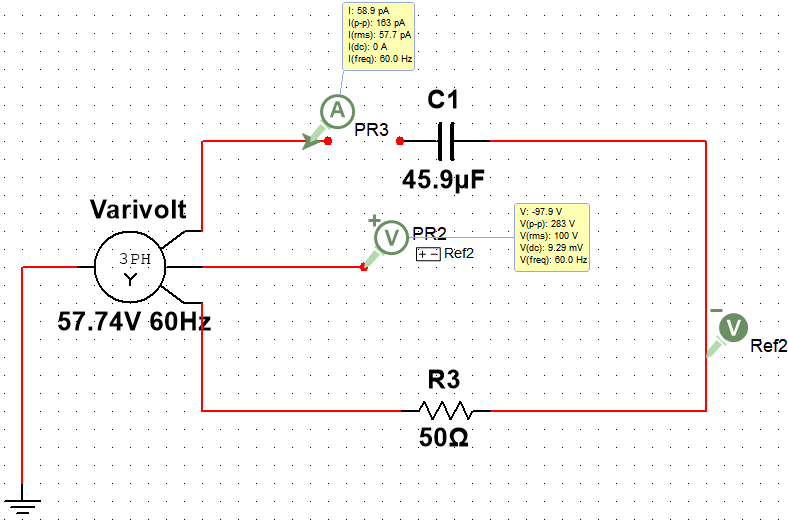
\includegraphics[width=13cm]{m2-sim-cba}
\caption{Simulação para determinação de sequência de fase CBA.}
\label{m2:sim:cba}
\end{figure}

\vspace{1cm}
\subsubsection{Verificação da sequência de fases - Fase C aberta}
\begin{figure}[H]
\centering
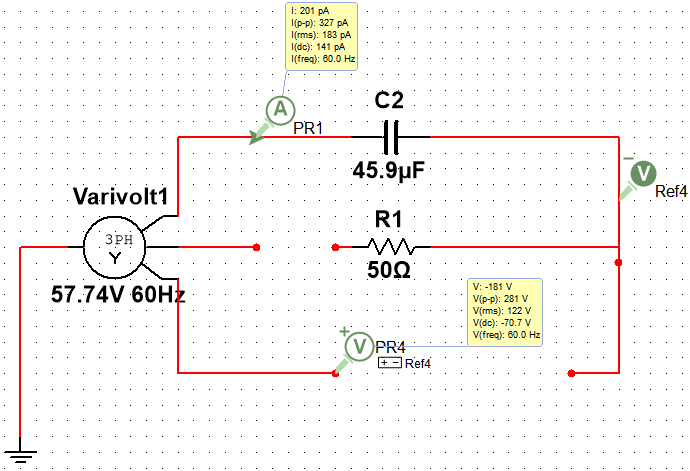
\includegraphics[width=13cm]{m3-sim-abc}
\caption{Método do voltímetro, utilizando-se equipamento digital.}
\label{m3:sim:abc}
\end{figure}

\vspace{0.2cm}
\begin{figure}[H]
\centering
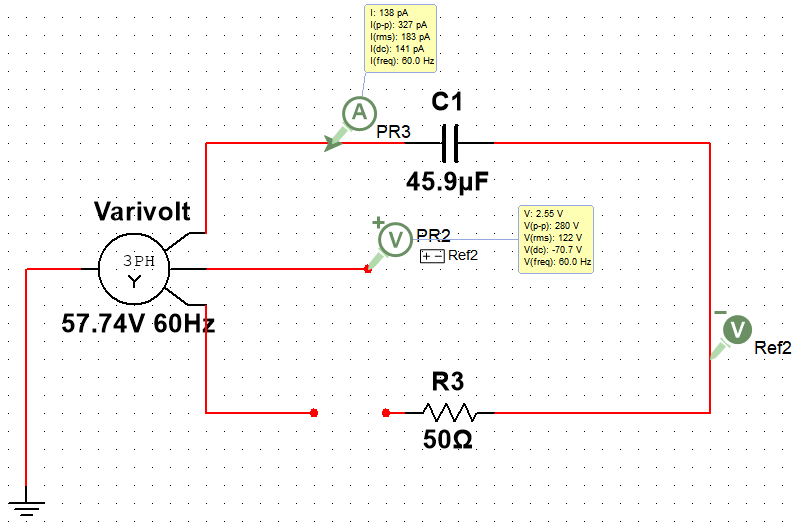
\includegraphics[width=13cm]{m3-sim-cba}
\caption{Simulação para determinação de sequência de fase CBA.}
\label{m3:sim:cba}
\end{figure}

\vspace{2cm}
\section{Conclusões} % (no mínimo 10 linhas) (5%);
Ter conhecimento sobre a sequência de fases em circuito equilibrado é de extrema importância, uma vez que do desequíbrio pode resultar correntes elevadas em determinada fase e assim danificar algum equipamento, além de ser essencial na determinação da direção de rotação de uma motor de indução
conectado à fonte de tensão trifásica. Para isso, tem-se equipamentos como o fasímetro e o sequencímetro. Entretanto, na ausência desses equipamentos sofisticados, o engenheiro deve ser capaz de determinar a sequência de fases utilizando-se de equipamentos de menor custo, como o voltímetro ou visualizando-se a intensidade do brilhar de uma lâmpada.

Assim, neste experimento é tratado o método dos voltímetros, e verificou-se que considera-se sequência de fases ABC, no caso de tensão na fase B $V_{bn'}>V_{ab}$. Enquanto que para $V_{bn'}<V_{ab}$ considera-se sequência de fases CBA. A conclusão do experimento terminou na verificação do mesmo efeito, porém utilizando-se lâmpadas nos terminais $V_{ab}$ e $V_{bn'}$, para visualizar o mesmo efeito na intensidade do brilhar.

\newpage
\begin{thebibliography}{9} 
% Introdução
\bibitem{PH}
    P. H. O. Rezende,
    "Circuitos Polifásicos Desequilibrados", 2018.

\bibitem{safe}
    SafetyTrabi,
    “Óculos de segurança: Saiba quando utilizar este EPI”, SafetyTrab, 2019.
 Disponível em:
 \url{https://www.safetytrab.com.br/blog/oculos-de-seguranca/}. Acesso em: ago. 2019.

\bibitem{UNIR}
    B. M. Nascimento, J. Carneiro, P. Viecilli,
    “Sequencímetro de Baixo Custo”, Fundação Universidade Federal de Rondônia - UNIR.
 Disponível em:
 \url{https://brunomarquesunir.wixsite.com/sequencimetro}. Acesso em: dez. 2019.

\bibitem{fig1}
    Dutra Máquinas.
 Disponível em:
 \url{https://m.dutramaquinas.com.br/p/fasimetro-com-indicador-led-690-volts-mfa-862-mfa-862}. Acesso em: dez. 2019.


\end{thebibliography}
\end{document}
